\chapter{المعايرة بقياس pH وبقياس الموصلية}\label{ch:g12:ph-conductivity-titrations}

تحمل قارورة خل خمر لصاقة «حموضة 6 \%»: أي ستة غرامات من
حمض الإيثانويك في كل مئة غرام من الخل. ولا حمض الإيثانويك
ولا قاعدته المرافقة ملوّن، ولن تنفع البرمنغنات هنا.
لكن \omterm{def:g9:acids-bases-ph:ph-paper}{مقياس pH} مغموسًا في الخل، أو خلية تقيس مدى
توصيله، يتابع التفاعل مع قاعدة قطرةً قطرةً، وشكل
المنحنى يبيّن بالضبط موضع \omterm{def:g11:titration:equivalence}{التكافؤ}. عشر دقائق على
طاولة المختبر، فيُتحقق من اللصاقة.

\begin{recall}
\omterm{def:g11:titration:titration}{المعايرة}، وتكافؤها \omterm{def:g11:titration:equivalence}{وحجم التكافؤ}
(\cref{ch:g11:titration})؛ وثوابت الحمضية (\cref{ch:g12:ka-and-pka})؛
وعلاقة هندرسون والكواشف الملوّنة
(\cref{ch:g12:buffers-predominance})؛ ومحاليل \omterm{def:g9:ions:ion}{الأيونات} توصل
الكهرباء (\cref{ch:g9:ions}).
\end{recall}

\begin{omfigure}
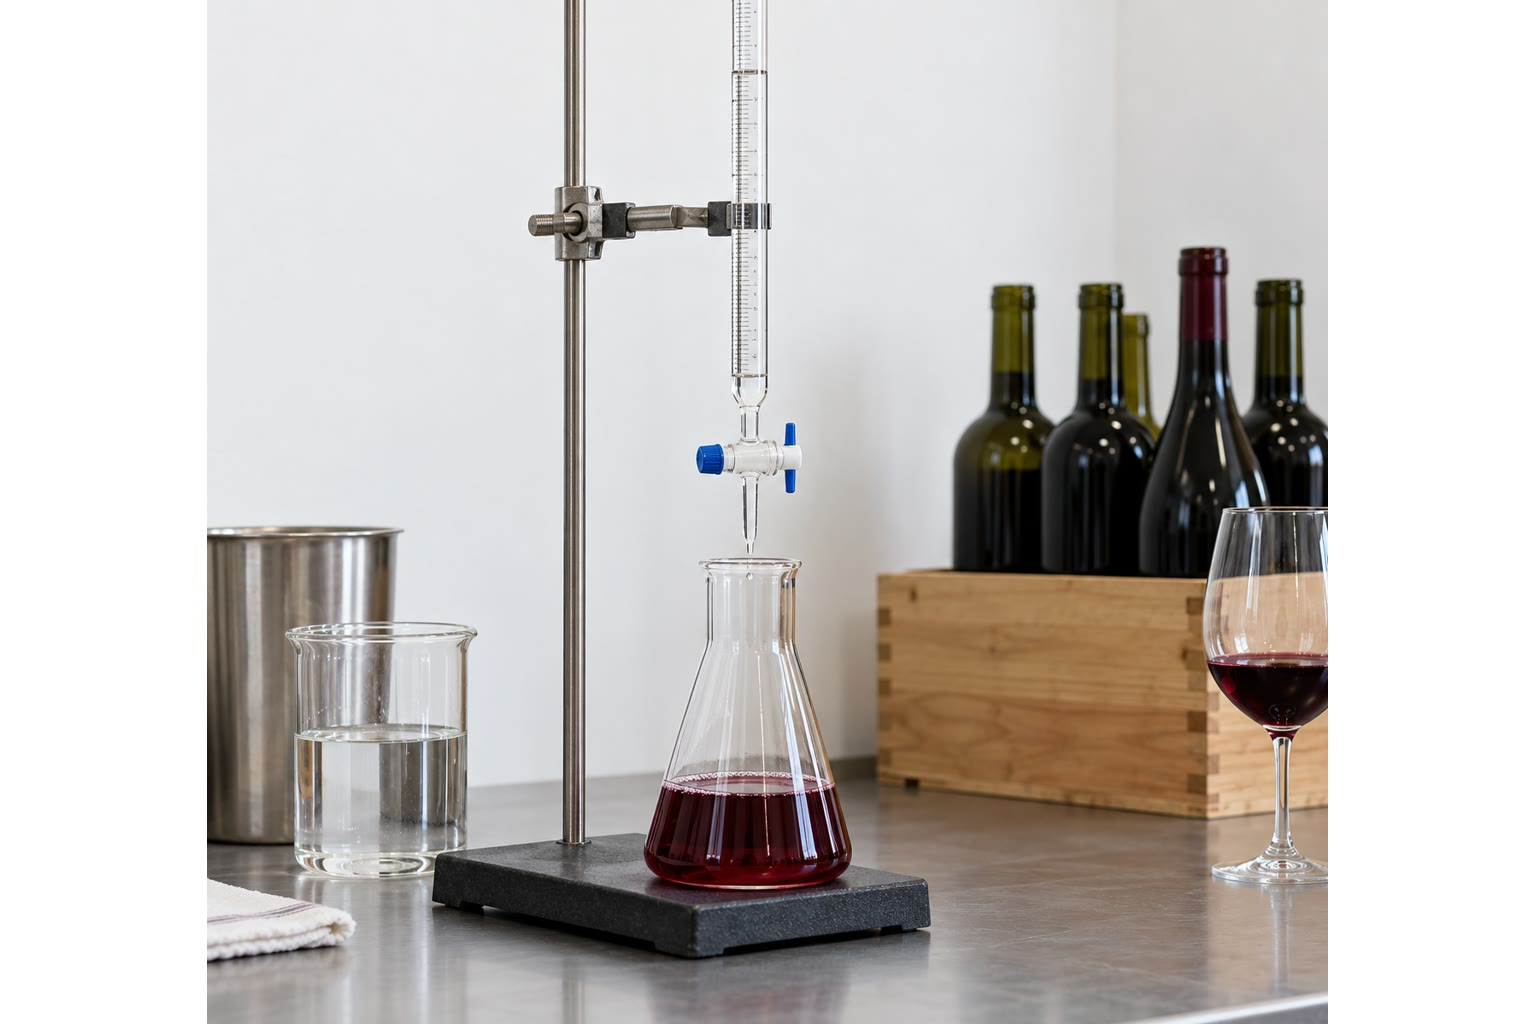
\includegraphics[width=0.45\linewidth]{images/book1/ai/g12-wine-lab.jpg}

{\small طاولة \omterm{def:g11:titration:titration}{معايرة} لدى صانع خمور.}
\end{omfigure}

\section{المعايرة بقياس pH}

\begin{definition}[المعايرة بقياس pH، نصف التكافؤ]\label{def:g12:ph-conductivity-titrations:ph-metric}
في \emph{المعايرة بقياس pH}\index{معايرة بقياس pH} تُقاس قيمة \omterm{def:g9:acids-bases-ph:ph}{pH}
\omterm{def:g11:titration:titration}{المحلول المراد معايرته} بعد كل إضافة من \omterm{def:g11:titration:titration}{المحلول المعايِر}، ويُرسم
منحنى \omterm{def:g9:acids-bases-ph:ph}{pH} بدلالة الحجم المضاف. و\emph{نصف التكافؤ}\index{نصف التكافؤ}
هو النقطة التي يكون قد أضيف عندها نصف \omterm{def:g11:titration:equivalence}{حجم التكافؤ}.
\end{definition}

\begin{omfigure}
\begin{tikzpicture}[font=\small, scale=0.65]
  \pic[transform shape] at (0,0) {stand={6.3}{2.0}};
  \pic[transform shape] at (2.0,0.68) {stirrer};
  \pic[transform shape] at (2.0,0.68) {beaker={0.45}{omWater}};
  \pic[transform shape] at (2.0,2.9) {burette={0.8}{omWater}};
  \pic[transform shape] (pr) at (2.6,0.95) {probe};
  \pic[transform shape] (m) at (6.4,3.4) {meter={pH}};
  \draw[black!70, thick] (pr-top) .. controls +(0,1.0) and +(0,-1.2) .. (m-a);
  \draw[omProp, thick, <-] (2.35,7.2) -- (4.3,7.6) node[right, text=black] {\foreignlanguage{arabic}{السحاحة: \babelsublr{NaOH}}};
  \draw[omProp, thick, <-] (1.4,1.1) -- (-1.4,1.6) node[left, text=black, align=right] {الحمض المراد معايرته};
  \draw[omProp, thick, <-] (2.75,2.4) -- (4.3,2.0) node[right, text=black] {\foreignlanguage{arabic}{مسبار \babelsublr{pH}}};
\end{tikzpicture}

{\small \omterm{def:g12:ph-conductivity-titrations:ph-metric}{معايرة بقياس pH}: المسبار مغموس في \omterm{def:g2:mixing-and-dissolving:dissolve}{المحلول} المُحرَّك،
والمقياس يبيّن قيمة \omterm{def:g9:acids-bases-ph:ph}{pH} بعد كل إضافة.}
\end{omfigure}

\begin{inthelab}[معايرة مقياس pH]
قبل الاستعمال، يُشطف المسبار بالماء المقطر ويُغمس في محلولين
منظِّمين معروفي قيمة \omterm{def:g9:acids-bases-ph:ph}{pH}، عادةً 7.0 و4.0 (أو 10.0): ويُضبط المقياس
ليقرأ قيمتيهما. وبين \omterm{def:g2:mixing-and-dissolving:dissolve}{محلول} وآخر يُشطف المسبار
ويُجفَّف بلطف بالربت، دون مسح أبدًا؛ ويُحفظ وطرفه رطب.
\end{inthelab}

\begin{omfigure}
\begin{minipage}{0.49\linewidth}
\begin{tikzpicture}
\begin{axis}[width=\linewidth, height=6cm, xmin=0, xmax=30, ymin=0, ymax=14,
    xlabel={\babelsublr{$V_{\text{NaOH}}$ (\si{mL})}}, ylabel={\babelsublr{pH}}, axis lines*=left,
    ymajorgrids, grid style={gray!20}, tick label style={font=\scriptsize},
    label style={font=\small}, title={\small \foreignlanguage{arabic}{\ce{HCl} بواسطة \ce{NaOH}}},
    title style={yshift=-4pt}]
  \addplot[very thick, omDef] table[x=V, y=pH] {figdata/out/grade-12-ph-conductivity-titrations-a.dat};
  \addplot[thick, omProp, densely dotted] table[x=V, y expr=\thisrow{dpH}/4]
    {figdata/out/grade-12-ph-conductivity-titrations-a.dat};
  \addplot[dashed, black!60] coordinates {(20,0) (20,7)};
  \node[font=\scriptsize, anchor=north west] at (axis cs:20.3,6.5) {$V_E = 20.0$};
\end{axis}
\end{tikzpicture}
\end{minipage}\hfill
\begin{minipage}{0.49\linewidth}
\begin{tikzpicture}
\begin{axis}[width=\linewidth, height=6cm, xmin=0, xmax=16, ymin=0, ymax=14,
    xlabel={\babelsublr{$V_{\text{NaOH}}$ (\si{mL})}}, ylabel={\babelsublr{pH}}, axis lines*=left,
    ymajorgrids, grid style={gray!20}, tick label style={font=\scriptsize},
    label style={font=\small}, title={\small \foreignlanguage{arabic}{\ce{CH3COOH} بواسطة \ce{NaOH}}},
    title style={yshift=-4pt}]
  \addplot[very thick, omDef] table[x=V, y=pH] {figdata/out/grade-12-ph-conductivity-titrations-b.dat};
  \addplot[thick, omProp, densely dotted] table[x=V, y expr=\thisrow{dpH}/4]
    {figdata/out/grade-12-ph-conductivity-titrations-b.dat};
  \addplot[dashed, black!60] coordinates {(10.1,0) (10.1,8.7)};
  \addplot[dashed, black!60] coordinates {(0,4.76) (5.05,4.76) (5.05,0)};
  \node[font=\scriptsize, anchor=south west] at (axis cs:0.2,4.8) {$pK_a = 4.76$};
  \node[font=\scriptsize, anchor=north west] at (axis cs:10.4,3.0) {$V_E = 10.1$};
\end{axis}
\end{tikzpicture}
\end{minipage}

{\small منحنيات \omterm{def:g9:acids-bases-ph:ph}{pH} محسوبة (بالأزرق) ومشتقها $d\mathrm{pH}/dV$
(بالبرتقالي، منقّطًا، مقسومًا على 4). يسارًا: \qty{20.0}{mL} من حمض الهيدروكلوريك
بتركيز \qty{0.100}{mol/L}؛ \omterm{def:g11:titration:equivalence}{والتكافؤ} عند \omterm{def:g9:acids-bases-ph:ph}{pH} 7.00. يمينًا: \qty{10.0}{mL} من
خل مخفف؛ عند \omterm{def:g12:ph-conductivity-titrations:ph-metric}{نصف التكافؤ} تساوي قيمة \omterm{def:g9:acids-bases-ph:ph}{pH} قيمة $pK_a$،
ويقع \omterm{def:g11:titration:equivalence}{التكافؤ} عند \omterm{def:g9:acids-bases-ph:ph}{pH} قاعدية.}
\end{omfigure}


\begin{method}[طريقة المشتقة]\label{met:g12:ph-conductivity-titrations:derivative}
احسب، بين قياسين متتاليين، الميل
$\Delta\mathrm{pH}/\Delta V$، وارسمه بدلالة $V$ (يقوم بذلك جدول بيانات أو
آلة حاسبة). \omterm{def:g11:titration:equivalence}{وحجم التكافؤ} هو حيث يكون هذا الميل
أكبر ما يمكن: قمة منحنى المشتقة.
\end{method}

\begin{method}[طريقة المماسات]\label{met:g12:ph-conductivity-titrations:tangent}
\begin{enumerate}
  \item ارسم مماسين متوازيين للمنحنى، أحدهما قبل القفزة والآخر بعدها،
        على جانبيها.
  \item ارسم المستقيم الموازي لهما في منتصف المسافة بينهما.
  \item نقطة تقاطعه مع المنحنى هي نقطة \omterm{def:g11:titration:equivalence}{التكافؤ}: اقرأ $V_E$ (وقيمة
        \omterm{def:g9:acids-bases-ph:ph}{pH} عند \omterm{def:g11:titration:equivalence}{التكافؤ}).
\end{enumerate}
\end{method}

\begin{proposition}[عند نصف التكافؤ، $\mathrm{pH} = pK_a$]\label{prop:g12:ph-conductivity-titrations:half}
في \omterm{def:g11:titration:titration}{معايرة} \omterm{def:g12:ka-and-pka:strong-acid}{حمض ضعيف} \ce{HA} \omterm{def:g12:ka-and-pka:strong-acid}{بقاعدة قوية}، يكون عند
\omterm{def:g12:ph-conductivity-titrations:ph-metric}{نصف التكافؤ} $\mathrm{pH} = pK_a$.
\end{proposition}

\begin{proof}
التفاعل \ce{HA + OH- -> A- + H2O} تام. وعند \omterm{def:g12:ph-conductivity-titrations:ph-metric}{نصف التكافؤ} يكون نصف
الحمض قد تحول إلى \ce{A-}: $[\ce{A-}] = [\ce{HA}]$،
وعلاقة هندرسون تعطي $\mathrm{pH} = pK_a + \log 1 = pK_a$.
\end{proof}

\begin{remark}[اختيار كاشف ملوّن انطلاقًا من المنحنى]\label{rem:g12:ph-conductivity-titrations:indicator}
% ledger: ind:BBT, ind:phenolphthalein
يجب أن يتغير لون الكاشف داخل القفزة. ففي حالة حمض الهيدروكلوريك
تمتد القفزة من نحو \omterm{def:g9:acids-bases-ph:ph}{pH} 4 إلى 10 فتناسب كواشف كثيرة، وأفضلها أزرق البروموثيمول؛
وفي حالة حمض الإيثانويك تكون القفزة أقصر وقاعدية، نحو 7 إلى 11:
فيناسبها الفينول فثالين (8.0--10.0)، أما أزرق البروموثيمول فيتغير لونه
مبكرًا جدًا.
\end{remark}

\section{الموصلية والمعايرة بقياس الموصلية}

\begin{definition}[الموصلية، الموصلية المولية الأيونية]\label{def:g12:ph-conductivity-titrations:conductivity}
\emph{الموصلية}\index{موصلية} $\sigma$ \omterm{def:g2:mixing-and-dissolving:dissolve}{لمحلول}
تقيس مدى توصيله للكهرباء؛ وتُقرأ على مقياس الموصلية
بالوحدة \si{mS/cm} (أو \si{S/m}). وكل \omterm{def:g9:ions:ion}{أيون} $i$ يسهم فيها
بما يتناسب مع تركيزه، بمعامل $\lambda_i$، هو
\emph{موصليته المولية الأيونية}\index{موصلية مولية أيونية}.
\end{definition}

\begin{proposition}[قانون كولراوش]\label{prop:g12:ph-conductivity-titrations:kohlrausch}
% ledger: lam:H+, lam:OH-, lam:Na+, lam:Cl-
\omterm{def:g2:mixing-and-dissolving:dissolve}{لمحلول} مخفف، $\sigma = \sum_i \lambda_i [X_i]$. وعند
\qty{25}{\celsius}، بالوحدة \si{S.cm^2/mol}: \ce{H3O+} 349.8، و\ce{OH-} 198.3،
و\ce{Cl-} 76.2، و\ce{Na+} 50.3. \omterm{def:g9:ions:ion}{فأيونات} الأكسونيوم والهيدروكسيد توصل
أفضل بكثير من كل \omterm{def:g9:ions:ion}{الأيونات} الأخرى.
\end{proposition}

\begin{proof}
نقبله (مجلد السنة الأولى). وقيمتا \ce{Cl-} و\ce{Na+} مستنتجتان من
الموصليتين المقيستين لمحلولي حمض الهيدروكلوريك وكلوريد الصوديوم،
بعد طرح \omterm{def:g12:ph-conductivity-titrations:conductivity}{موصلية} \ce{H3O+} منهما.
\end{proof}

\begin{definition}[المعايرة بقياس الموصلية]\label{def:g12:ph-conductivity-titrations:conductimetric}
في \emph{المعايرة بقياس الموصلية}\index{معايرة بقياس الموصلية}
تُقاس \omterm{def:g12:ph-conductivity-titrations:conductivity}{الموصلية} بعد كل إضافة من \omterm{def:g11:titration:titration}{المحلول المعايِر}. ويُخفَّف \omterm{def:g11:titration:titration}{المحلول
المراد معايرته} في حجم كبير من الماء، بحيث لا يكاد الحجم
المضاف يغيّره: فتقع النقاط عندئذ على خطوط مستقيمة، يتغير
ميلها عند \omterm{def:g11:titration:equivalence}{التكافؤ}.
\end{definition}

\begin{omfigure}
\begin{minipage}{0.4\linewidth}\centering
\begin{tikzpicture}[font=\small, scale=0.75]
  \pic[transform shape] at (0,0) {beaker={0.6}{omWater}};
  \pic[transform shape] (cc) at (0.2,0.2) {condcell};
  \pic[transform shape] (m) at (2.6,3.4) {meter={mS/cm}};
  \draw[black!70, thick] (cc-top) .. controls +(0,0.8) and +(0,-1) .. (m-a);
  \node[anchor=north, align=center] at (0.6,-0.15) {خلية قياس الموصلية\\ في المحلول};
\end{tikzpicture}
\end{minipage}\hfill
\begin{minipage}{0.56\linewidth}
\begin{tikzpicture}
\begin{axis}[width=\linewidth, height=5.4cm, xmin=0, xmax=20, ymin=0,
    ymax=4.6, xlabel={\babelsublr{$V_{\text{NaOH}}$ (\si{mL})}}, ylabel={\babelsublr{$\sigma$ (\si{mS/cm})}},
    axis lines*=left, ymajorgrids, grid style={gray!20},
    tick label style={font=\scriptsize}, label style={font=\small}]
  \addplot[only marks, mark=*, mark size=1.4pt, omDef] table[x=V, y=sigma]
    {figdata/out/grade-12-ph-conductivity-titrations-c.dat};
  \addplot[dashed, black!60] coordinates {(10,0) (10,4.6)};
  \node[font=\scriptsize, anchor=south west] at (axis cs:10.3,0.2) {$V_E = 10.0$};
\end{axis}
\end{tikzpicture}
\end{minipage}

{\small يسارًا: خلية قياس \omterm{def:g12:ph-conductivity-titrations:conductivity}{الموصلية}. يمينًا: \qty{100}{mL} من حمض
الهيدروكلوريك بتركيز \qty{0.0100}{mol/L} يعايَر بهيدروكسيد الصوديوم بتركيز
\qty{0.100}{mol/L} (محسوب بقانون كولراوش). تنخفض \omterm{def:g12:ph-conductivity-titrations:conductivity}{الموصلية}
ثم ترتفع: مستقيمان يلتقيان عند \omterm{def:g11:titration:equivalence}{التكافؤ}.}
\end{omfigure}

\begin{example}[قراءة المستقيمين]\label{ex:g12:ph-conductivity-titrations:lines}
قبل \omterm{def:g11:titration:equivalence}{التكافؤ}، كل \omterm{def:g9:ions:ion}{أيون} \ce{OH-} يضاف يزيل \omterm{def:g9:ions:ion}{أيون} \ce{H3O+}
($\lambda = 349.8$) ويأتي \omterm{def:g9:ions:ion}{بأيون} \ce{Na+} ($\lambda = 50.3$): فتنخفض
\omterm{def:g12:ph-conductivity-titrations:conductivity}{الموصلية} بشدة. وبعد \omterm{def:g11:titration:equivalence}{التكافؤ}، تتراكم \omterm{def:g9:ions:ion}{أيونات} \ce{Na+} و\ce{OH-}
($\lambda = 198.3$) فحسب: فترتفع. ويلتقي المستقيمان عند
$V_E = \qty{10.0}{mL}$، إذن كان تركيز الحمض
$0.100 \times 10.0 / 100 = \qty{0.0100}{mol/L}$.
\end{example}

\begin{method}[التكافؤ من معايرة بقياس الموصلية]\label{met:g12:ph-conductivity-titrations:two-lines}
ارسم أفضل مستقيم يمر بالنقاط التي قبل \omterm{def:g11:titration:equivalence}{التكافؤ}
وأفضل مستقيم يمر بالنقاط التي بعده؛ واقرأ $V_E$ عند
تقاطعهما. وتُستبعد النقاط القريبة من \omterm{def:g11:titration:equivalence}{التكافؤ}، حيث ينحني الخطان.
\end{method}

\begin{remark}[أي طريقة ومتى]\label{rem:g12:ph-conductivity-titrations:which}
\omterm{def:g12:buffers-predominance:indicator}{الكاشف الملوّن} أسرع الطرق حين يوجد كاشف مناسب. \omterm{def:g12:ph-conductivity-titrations:ph-metric}{والمعايرة بقياس pH}
تعطي أيضًا قيمة $pK_a$ \omterm{def:g12:ka-and-pka:strong-acid}{الحمض الضعيف}، وتصلح للمحاليل الملوّنة
أو العكرة. \omterm{def:g12:ph-conductivity-titrations:conductimetric}{والمعايرة بقياس الموصلية} لا تحتاج إلى قفزة في \omterm{def:g9:acids-bases-ph:ph}{pH}
إطلاقًا: فهي تصلح للأحماض الشديدة الضعف أو الشديدة \omterm{def:g10:concentration-and-dilution:dilution}{التخفيف}، ولتفاعلات
الترسيب، ما دامت \omterm{def:g9:ions:ion}{الأيونات} تتغير.
\end{remark}

\begin{safety}{\ghs[0.82cm]{GHS05}\ghs[0.82cm]{GHS07}}
% ledger: ghs:NaOH
محاليل هيدروكسيد الصوديوم تحرق الجلد والعينين، حتى المخففة منها
في العينين: نظارتان واقيتان طوال الوقت، وكل رذاذ يُشطف فورًا بكثير
من الماء.
\end{safety}

\section{تمارين}


\begin{exercise}[$\star$]\label{exo:g12:ph-conductivity-titrations:1}
اقرأ \omterm{def:g11:titration:equivalence}{حجم التكافؤ} على منحنى حمض الهيدروكلوريك المعايَر بهيدروكسيد
الصوديوم بتركيز \qty{0.100}{mol/L}، واستنتج تركيز
\qty{20.0}{mL} من الحمض.
\end{exercise}

\begin{exercise}[$\star$]\label{exo:g12:ph-conductivity-titrations:2}
يُعايَر \omterm{def:g12:ka-and-pka:strong-acid}{حمض ضعيف} بهيدروكسيد الصوديوم؛ $V_E = \qty{12.0}{mL}$. وعند
\qty{6.0}{mL} تكون قيمة \omterm{def:g9:acids-bases-ph:ph}{pH} 3.75. أعطِ $pK_a$ الحمض. وأي حمض من
أحماض سلّم $pK_a$ قد يكون؟
\end{exercise}

\begin{exercise}[$\star$]\label{exo:g12:ph-conductivity-titrations:3}
أي \omterm{def:g12:buffers-predominance:indicator}{كاشف ملوّن} تختار \omterm{def:g11:titration:titration}{لمعايرة} حمض الإيثانويك بهيدروكسيد
الصوديوم؟ ولماذا لا تختار أحمر الميثيل؟
\end{exercise}

\begin{exercise}[$\star$]\label{exo:g12:ph-conductivity-titrations:4}
لماذا يجب معايرة \omterm{def:g9:acids-bases-ph:ph-paper}{مقياس pH} قبل استعماله؟ وبماذا؟
\end{exercise}

\begin{exercise}[$\star$]\label{exo:g12:ph-conductivity-titrations:5}
مستعينًا بالموصليات المولية الأيونية، رتّب \omterm{def:g9:ions:ion}{الأيونات} \ce{H3O+}، و\ce{OH-}،
و\ce{Na+}، و\ce{Cl-} من الأفضل توصيلًا إلى الأسوأ.
\end{exercise}

\begin{exercise}[$\star\star$]\label{exo:g12:ph-conductivity-titrations:6}
يتطلب \qty{20.0}{mL} من \omterm{def:g2:mixing-and-dissolving:dissolve}{محلول} حمض الإيثانويك \qty{14.6}{mL} من
هيدروكسيد الصوديوم بتركيز \qty{0.050}{mol/L}. احسب تركيزه.
\end{exercise}

\begin{exercise}[$\star\star$]\label{exo:g12:ph-conductivity-titrations:7}
القراءات قرب \omterm{def:g11:titration:equivalence}{التكافؤ} هي: \qty{9.6}{mL}، \omterm{def:g9:acids-bases-ph:ph}{pH} 5.7؛
\qty{9.8}{mL}، 6.1؛ \qty{10.0}{mL}، 7.0؛ \qty{10.2}{mL}، 10.5؛
\qty{10.4}{mL}، 11.0. احسب $\Delta\mathrm{pH}/\Delta V$ بين
النقاط المتتالية وحدد موضع $V_E$.
\end{exercise}

\begin{exercise}[$\star\star$]\label{exo:g12:ph-conductivity-titrations:8}
في \omterm{def:g12:ph-conductivity-titrations:conductimetric}{المعايرة بقياس الموصلية} لحمض الهيدروكلوريك، اشرح إشارة
الميل قبل \omterm{def:g11:titration:equivalence}{التكافؤ} وبعده، مستعينًا \omterm{def:g9:ions:ion}{بالأيونات} الموجودة.
\end{exercise}

\begin{exercise}[$\star\star$]\label{exo:g12:ph-conductivity-titrations:9}
ارسم شكلًا تقريبيًا لمنحنى \omterm{def:g12:ph-conductivity-titrations:conductimetric}{المعايرة بقياس الموصلية} لحمض الإيثانويك المعايَر بهيدروكسيد
الصوديوم. ولماذا ترتفع \omterm{def:g12:ph-conductivity-titrations:conductivity}{الموصلية} حتى قبل \omterm{def:g11:titration:equivalence}{التكافؤ}؟
\end{exercise}

\begin{exercise}[$\star\star$]\label{exo:g12:ph-conductivity-titrations:10}
على المنحنى المحسوب للخل المخفف، اقرأ قيمة \omterm{def:g9:acids-bases-ph:ph}{pH} في البداية،
وعند \omterm{def:g12:ph-conductivity-titrations:ph-metric}{نصف التكافؤ} وعند \omterm{def:g11:titration:equivalence}{التكافؤ}. ولماذا تكون قيمة \omterm{def:g9:acids-bases-ph:ph}{pH} الابتدائية أعلى بكثير
من قيمة \omterm{def:g9:acids-bases-ph:ph}{pH} حمض الهيدروكلوريك بالتركيز نفسه؟
\end{exercise}

\begin{exercise}[$\star\star$]\label{exo:g12:ph-conductivity-titrations:11}
لماذا يُخفَّف \omterm{def:g11:titration:titration}{المحلول المراد معايرته} في حجم كبير من الماء قبل
\omterm{def:g12:ph-conductivity-titrations:conductimetric}{المعايرة بقياس الموصلية}؟
\end{exercise}

\begin{exercise}[$\star\star\star$]\label{exo:g12:ph-conductivity-titrations:12}
يحوي \omterm{def:g2:mixing-and-dissolving:dissolve}{محلول} حمض الهيدروكلوريك وحمض الإيثانويك معًا. ويُعايَر
بهيدروكسيد الصوديوم مع قياس قيمة \omterm{def:g9:acids-bases-ph:ph}{pH}. اشرح لماذا يُظهر
المنحنى قفزتين، وماذا يقيس كل من حجمي \omterm{def:g11:titration:equivalence}{التكافؤ}.
\end{exercise}

\begin{exercise}[$\star\star\star$]\label{exo:g12:ph-conductivity-titrations:13}
احسب \omterm{def:g12:ph-conductivity-titrations:conductivity}{الموصلية} في بداية \omterm{def:g12:ph-conductivity-titrations:conductimetric}{المعايرة بقياس الموصلية} في
الفصل (حمض الهيدروكلوريك بتركيز \qty{0.0100}{mol/L}) وعند \omterm{def:g11:titration:equivalence}{التكافؤ}
(\qty{110}{mL} من \omterm{def:g2:mixing-and-dissolving:dissolve}{محلول} كلوريد الصوديوم). وقارن بالشكل.
\end{exercise}

\begin{exercise}[$\star\star\star$]\label{exo:g12:ph-conductivity-titrations:14}
\omterm{def:g9:acids-bases-ph:ph-paper}{مقياس pH} سيئ المعايرة يقرأ كل قيمة \omterm{def:g9:acids-bases-ph:ph}{pH} أعلى بمقدار 0.2. فما الخطأ الذي
يسببه في \omterm{def:g11:titration:equivalence}{حجم التكافؤ} \omterm{def:g12:ph-conductivity-titrations:ph-metric}{لمعايرة بقياس pH}؟ وفي قيمة $pK_a$
المقروءة عند \omterm{def:g12:ph-conductivity-titrations:ph-metric}{نصف التكافؤ}؟
\end{exercise}

\begin{exercise}[$\star\star\star$]\label{exo:g12:ph-conductivity-titrations:15}
لماذا تستطيع \omterm{def:g12:ph-conductivity-titrations:conductimetric}{المعايرة بقياس الموصلية} متابعة تفاعل \omterm{def:g9:ions:ion}{أيونات} الفضة
مع \omterm{def:g9:ions:ion}{أيونات} الكلوريد، \ce{Ag+ + Cl- -> AgCl(s)}، في حين لا تستطيع ذلك \omterm{def:g12:ph-conductivity-titrations:ph-metric}{المعايرة
بقياس pH}؟ صف المنحنى المتوقع حين تضاف نترات الفضة
إلى كلوريد الصوديوم (خذ $\lambda$ \omterm{def:g9:ions:ion}{للأيون} \ce{NO3-} قريبة من قيمتها \omterm{def:g9:ions:ion}{للأيون}
\ce{Cl-}).
\end{exercise}

\section{مسألة: أحموضة الخل 6\,\% حقًا؟}

\begin{problem}[{مسألة نهاية الأسبوع --- أيحوي خل لصاقته «حموضة 6 \%»
حقًا ستة غرامات من حمض الإيثانويك في كل مئة غرام؟}]
\label{pb:g12:ph-conductivity-titrations:1}
% ledger: pka:ethanoic, ind:phenolphthalein, lam:OH-, lam:Na+, aw:C, aw:H, aw:O
يُتحقق من خل لصاقته «حموضة 6 \%». يوزن \qty{100.0}{mL}
منه: \qty{101}{g}. ويُخفَّف الخل عشر مرات، ثم
يُعايَر \qty{10.0}{mL} من \omterm{def:g2:mixing-and-dissolving:dissolve}{المحلول} المخفف بهيدروكسيد الصوديوم
بتركيز \qty{0.100}{mol/L}، مع \omterm{def:g9:acids-bases-ph:ph-paper}{مقياس pH}؛ والمنحنى المحسوب في
الفصل (يمينًا) يطابق القياسات.

\medskip
\noindent\textbf{الجزء الأول --- تحضير العيّنة.}
\begin{enumerate}
  \item ماذا تعني «حموضة 6 \%»؟
  \item إذا كانت اللصاقة صحيحة، فما كتلة حمض الإيثانويك في
        \qty{100.0}{mL} من الخل؟ وما \omterm{def:g10:concentration-and-dilution:molar-concentration}{التركيز المولي}
        الموافق؟
  \item لماذا يُخفَّف الخل قبل \omterm{def:g11:titration:titration}{المعايرة}؟
  \item ما الأدوات الزجاجية المستعملة لتخفيفه عشر مرات؟
\end{enumerate}

\medskip
\noindent\textbf{الجزء الثاني --- \omterm{def:g12:ph-conductivity-titrations:ph-metric}{المعايرة بقياس pH}.}
\begin{enumerate}[resume]
  \item اكتب معادلة تفاعل \omterm{def:g11:titration:titration}{المعايرة}.
  \item اقرأ \omterm{def:g11:titration:equivalence}{حجم التكافؤ} على المنحنى.
  \item احسب تركيز الخل المخفف.
  \item استنتج تركيز الخل.
  \item اقرأ قيمة \omterm{def:g9:acids-bases-ph:ph}{pH} عند \omterm{def:g12:ph-conductivity-titrations:ph-metric}{نصف التكافؤ}. ماذا تعطي؟
  \item لماذا تكون قيمة \omterm{def:g9:acids-bases-ph:ph}{pH} عند \omterm{def:g11:titration:equivalence}{التكافؤ} أعلى من 7؟
  \item أي \omterm{def:g12:buffers-predominance:indicator}{كاشف ملوّن} كان سيعطي النتيجة نفسها؟
\end{enumerate}

\medskip
\noindent\textbf{الجزء الثالث --- تحقق بقياس \omterm{def:g12:ph-conductivity-titrations:conductivity}{الموصلية}.}
\begin{enumerate}[resume]
  \item تُعاد \omterm{def:g11:titration:titration}{المعايرة} بخلية قياس \omterm{def:g12:ph-conductivity-titrations:conductivity}{الموصلية}، والعيّنة
        مخففة في \qty{200}{mL} من الماء. أي \omterm{def:g9:ions:ion}{أيونات} تظهر في
        \omterm{def:g2:mixing-and-dissolving:dissolve}{المحلول} قبل \omterm{def:g11:titration:equivalence}{التكافؤ}؟
  \item لماذا ترتفع \omterm{def:g12:ph-conductivity-titrations:conductivity}{الموصلية} ببطء فقط قبل \omterm{def:g11:titration:equivalence}{التكافؤ}؟
  \item لماذا ترتفع أسرع بعده؟
  \item لماذا تكون \omterm{def:g12:ph-conductivity-titrations:conductivity}{الموصلية} منخفضة جدًا في البداية؟
  \item أين يجب أن يلتقي المستقيمان؟
\end{enumerate}

\medskip
\noindent\textbf{الجزء الرابع --- الحكم.}
\begin{enumerate}[resume]
  \item احسب \omterm{def:g10:concentration-and-dilution:mass-concentration}{التركيز الكتلي} لحمض الإيثانويك في الخل.
  \item احسب كتلة حمض الإيثانويك في \qty{100.0}{mL} من الخل.
  \item استنتج كتلة حمض الإيثانويك في كل \qty{100}{g} من الخل.
  \item اذكر الجواب النهائي: ما حموضة الخل؟
\end{enumerate}
\end{problem}
